\documentclass{project}
\usepackage[toc,page]{appendix}
\usepackage[pdfauthor={Sam - srj12, Nathan - naw21},pdftitle={Software Engineering Group Project, Design Specification},pdftex]{hyperref}

\usepackage{graphicx}
\usepackage{rotating}
\graphicspath{{images/}}
%use this where you need to include images after putting the image in the images folder
%\includegraphics[width=\textwidth]{filename}

%YOU SHOULDN't NEED TO EDIT THIS FILE, OTHER THAN TO ADD YOURSELF AS AUTHOR. or write intro or document history%

\title{Software Engineering Group Project}
\subtitle{Design Specification}
\author{
	Sam Jones - srj12, \newline
	Nathan Williams - naw21, \newline
    Rhys Evans - rhe24, \newline
    Alex Thumwood - alt38, \newline
    Aleksandra Madej - alm82, \newline
    Lampros Petridis - lap12, \newline
    Cameron Humphreys - cah27
}     
\shorttitle{Design Spec}
\version{1.0}
\status{Review}
\date{2018-03-08}
\configref{GP01-UIS-DS}

\begin{document}	
	\maketitle
	\tableofcontents
	\clearpage
	\section{INTRODUCTION} % Alex - DONE
		\subsection{Purpose of this Document}
        The purpose of this document is to describe in detail the implementation of the software JoggleCube. JoggleCube is a single player word finding game aimed a Second-Year computer science students. 
		\subsection{Scope}
        	This document describes the functions of the software 'JoggleCube' and the implementation of said functions, including the classes, interfaces and controllers used both in the back end and the UI of the software, and the relationships between entities within the software. It also provides an explanation of the algorithms used in the implementation of the software's logic and examples of some of the data input/output from the class methods using these algorithms. It should be read in the context of the Jogglecube Requirements Specification [SE.QA.CSRS] in regards to required functionalities. 
     
		\subsection{Objectives}
			This Document aims to:
			\begin{itemize}
				\item  Describe the overall structure of the JoggleCube application, in terms of classes, interfaces and controllers.
                \item Describe how each feature of the application has been implemented, and how these features match the requirements specified in SE.QA.CSRS.
                \item Describe exactly how the software works at runtime, with relevant diagrams. 
                
			\end{itemize}
	\section{DECOMPOSITION DESCRIPTION}
	\subsection{Programs in system}
    There is only one part of this program that can effectively be called a program and that is the overall JoggleCube program itself.
    	\subsubsection{JoggleCube}
        The only part of this project that you could effectively call a program is the JoggleCube program itself, which is an all-encompassing, all performing program that does everything that is set forth in the functional requirements of this document. The Program runs using Java 1.8 and up when compiled and will effectively be the game program, it pops up in a window where you can play JoggleCube.
	\subsection{Significant classes in each program}
    Since there is only one program present in the project I will be discussing the major classes of the JoggleCube program.
		\subsubsection{Significant classes in JoggleCube}
        There will be 6 major classes present in the JoggleCube program, namely Main, JoggleCube, Start, Game and End.
        	\paragraph{Main}
            Main is the class in which the program is launched and you will find that this class is used primarily as a method of loading in different resources for the program and making sure that the correct objects have been created together. In essence, this is the major backbone of the program. It creates the backbones of both frontend and backend and allows the main part of the program to be actually relatively tidy when it comes to everything working together.
            \paragraph{JoggleCube}
            JoggleCube is the main class that handles all backend communication with the front end. If you need access to Dictionary, Timer, HighScores or any other backend feature you will need to go via this class. This class will handle both the start and end of the game and should be making sure that this is pushed to the front end, this class should also handle how any core back-end feature interacts with other core-backend features.
            \paragraph{Start}
            Start is where you can navigate to create a new gird, load a grid, change the grid language, view high scores and go to help screen. This is effectively the class that allows the game to start handling the front-end generation and handles the basic menu functionality of the game.
            \paragraph{Game}
            Game displays everything to do with the actual game and it does all the passing to the backend of the main gameplay. It also handles the creation of the timer and when the timer should stop and start. The Game is essentially the front-end game controller which handles the generation of the cube in different ways as well as the displaying of any in-game features.
            \paragraph{End}
            End handles the end game screen, giving you the restart option, the display of scores as well as saving and returning to the main menu, however not as central as other classes the End is main class as without it the game wouldn't properly end and a lot of functional requirements are missing.
	\subsection{Mapping from requirements to classes}
    	\begin{tabular}{|l|l|}
        	\hline
            Requirement & Classes providing requirement \\ \hline \hline
            FR1 &  Start\\ \hline
            FR2 & JoggleCube, Cube\\ \hline
            FR3 &  LoadGrid, JoggleCube, Cube\\\hline
            FR4 & GameTimer, JoggleCube\\ \hline
            FR5 & End\\ \hline
            FR6 & End, JoggleCube, Block\\ \hline
            FR7 & Game, GridDisplayer\\ \hline
            FR8 & Game\\ \hline
            FR9 & Game, GridDisplayer, JoggleCube\\ \hline
            FR10 & JoggleCube\\ \hline
            FR11 & JoggleCube\\ \hline
        \end{tabular} % Sam    - DONE
	\section{DEPENDENCY DESCRIPTION}
	\subsection{Component Diagrams}
		\subsubsection{Component Diagram for JoggleCube}
        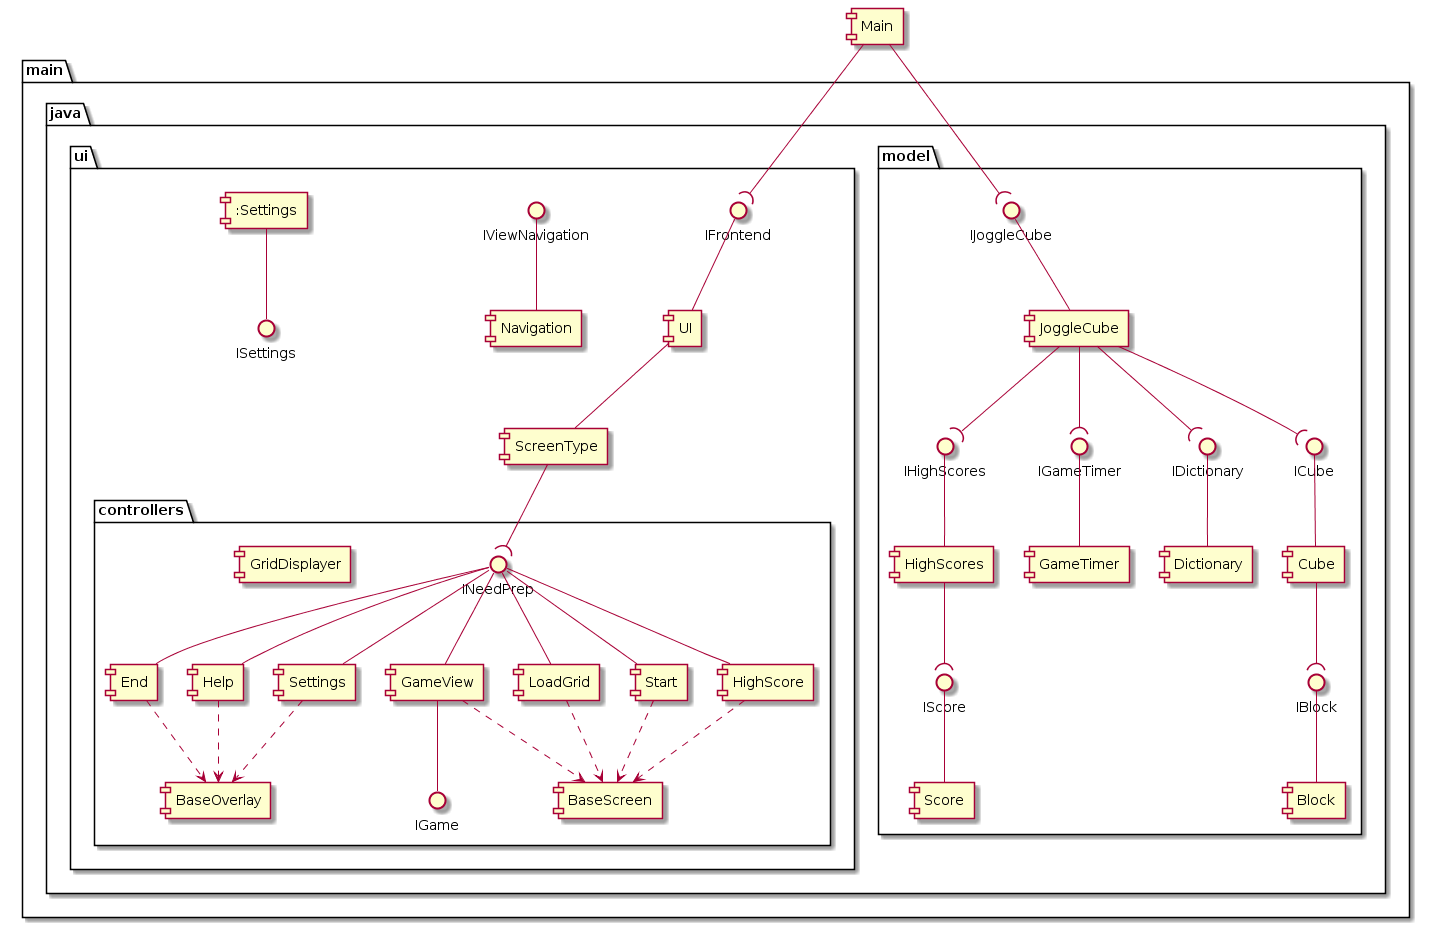
\includegraphics[width=18cm]{compdiag.png} % Alex 
	\section{INTERFACE DESCRIPTION}
	\subsection{Model}
		\subsubsection{JoggleCube interface specification}
        	This is the main class of the system, it is responsible for managing the logic of the game and it's behaviour. This class implements the singeton design pattern.
         \begin{itemize}
         	\item  public void generateRandomGrid() - A public method to generate a new random grid and initialize various game elements. 
            \item public boolean loadGrid(String filename) - A method to load all the data needed to create a grid from a file, this also loads all the highscores associated with a given grid.
            \item public boolean testWordValidity(String word) - A method to test if a inputted word is valid by doing a search of the Dictionary and checking if the word was already used.
            \item public String[][][] getCubeData() - A method to return the currently loaded grid data in a 3D String array representation.
            \item public ObservableList<IScore> getOverallHighScores() - A method that returns an unsorted ArrayList of overall high scores.
            \item public ObservableList<IScore> getCurrentCubeHighScores() - A method that returns an unsorted ArrayList of high scores for the currently loaded cube.
            \item pubic ObservableList<String> getAvailableGrids() - A method that returns a list of all the .grid files found in the 'saves' directory that are available for loading.
            \item public boolean saveGrid(String filename) - A method to save the current grid data to a file
            \item public void saveOverallScores() - A method to save the overall high scores of the game to a file.
            \item public void loadOverallScores() - A method to load all the overall highscores from a file and store in an ArrayList.
            \item public int getHighestScore() - A method to get the highest score value from the overall highscores ArrayList.
            \item public void setName(String name) - A method to set the name of the current user.
            \item public void startTimer() - A method to start the game timer to be called when the game starts.
            \item public void interruptTimer() - A method to stop the game timer.
            \item public void setLanguage(String lang) - A method to set the current language of the grid.
            \item public int getWordScore(String word) - A method to get the score value of a given word.
            \item public int getScore() - A method to return the user's current score.
            \item public void loadNewDictionary() - A method to Load a dictionary of the currently selected language.
            \item public void resetGameState() - A method to re-initialize the game when a new game is started.
         \end{itemize}
        
        
		\subsubsection{Dictionary interface specification} %Aleksandra    
        This public class is responsible for handling dictionary of valid words that can be created in the game, including loading and searching it.
        \begin{itemize}
        \item Dictionary() - creates an empty Dictionary object
\item  int getDictionarySize() - returns the size of dictionary HashMap
\item  void loadDictionary(String filename) - loads the dictionary from a file with the given name into the HashMap
\item boolean searchDictionary(String word) - takes a word as an argument and checks if it exists if the dictionary. Returns true if the HashMap contains the word and false otherwise.

	\end{itemize}
        \subsubsection{Block interface specification} % Aleksandra
        This public class is responsible for for handling single blocks in the cube.
        \begin{itemize}
        \item Block(String newLetter) - creates a new block containing a given letter
\item  void setLetter(String newLetter) - takes a new letter as an argument and sets a letter in a block to the new letter
\item  String getLetter() - returns the letter in a block

		\end{itemize}
        \subsubsection{Cube interface specification} % Aleksandra
        This public class is responsible for handling creation, loading and saving the cube in the game, as well as storing scores assigned to each letter in the cube.
        \begin{itemize}
        \item  Cube() - creates an empty Cube object
\item  Cube ( String letterFilename ) - creates a Cube object from a file with the given name. File should contain letters that cube can be filled with as well as maximum population and score for each letter
\item  ArrayList $\langle String\rangle$ getBagOfLetters() - returns an ArrayList containing maximum number of occurences of each letter that can be used to fill the cube
\item  Block getBlock(int x, int y, int z) - takes coordinates for each dimension and returns a single Block object at this position.
\item  Block[][][] getCube() - Returns a Cube as a multi-dimensional array of Block objects
\item  ArrayList$\langle int[ ] \rangle$ getNeighbours(int x, int y, int z) - takes coordinates of a block as arguments and returns an ArrayList of arrays containing coordinates of all adjacent blocks.
\item  HashMap $\langle String, String \rangle$ getScores() - returns a HashMap of letters and assigned to them scores
\item  boolean loadCube(Scanner file) - takes a file as an argument and fills the cube with letters from that file.
\item  void populateCube(String letterFilename) - takes a name of file containing letters, their population and scores and generates a random cube with those letters.
\item  boolean saveCube(PrintWriter file) - takes a file as an argument and saves cube data into it
\item  void setBlock(int x, int y, int z, Block block) - takes coordinates of a block and new block and sets block at given position to the new block
\item  void setLanguage(String language) - sets the language of the cube to the given language

        \end{itemize}
        \subsubsection{HighScores interface specification} % Lampros? and Sam.
        This public class is used to handle the high scores, loading, saving, setting and giving of the high scores is all handled by this class.
        \begin{itemize}
        	\item public void loadScores() - The way highscores are loaded is by calling loadScores in the HighScores class.  The specified file containing the scores is then located, the scores are read in and saved in the scores arraylist.
            \item public void saveScores() - The highscores are saved by calling saveScores in the HighScores class which then writes each score from the score arraylist to a file in a specified location using saveScore in the Score class.
            \item public void addScore() - An individual score can be added by calling addScore in the HighScores class. The score is then added to the score arraylist.
            \item public void getScore(int i) - The highest score can be returned by calling getHighestScore in the HighScores class which then sorts the arraylist and returns the highest score in record.
        \end{itemize}
        \subsubsection{Score interface specification} % Lampros? + Sam
        The score interface class implements the Score class. The interface class can return the date, the score, the name and as well as save the score to a file by calling methods from the score class.
        \begin{itemize}
        	\item getDate() - The way the date of a score is returned is by calling getDate in the Score class. The called method then returns the date of a given high score entry.
            \item getScore() - The value of a score can be returned by calling getScore in the Score class which then returns the score value of a given high score entry.
            \item getName() - The way the name of a score holder is returned is by calling getName in the Score clas which then returns the name of a given high score holder.
            \item saveScore() - A score can be saved in a file by calling saveScore in the Score class. The called method then prints the date, the score and the name in a specified file which then can be read in so that the score is loaded.
        \end{itemize}    
        \subsubsection{GameTimer interface specification} % Cameron
        This public class is responsible for the creation, running and termination of the in-game timer. The public methods within the class are as follows.
        \begin{itemize}
       		    \item public void setCurrentTime(Duration currentTime) - A public method that takes a single parameter 'currentTime'  which sets how long the timer will count down for.  currentTime is a Duration.
      		    \item public Duration getCurrentTime() - A public method that returns the Duration currentTIme.
     		    \item public boolean isInterrupt() - A public method returns a boolean that is used to check if the game timer has been interrupted.
   			    \item public void resetTime() - A public method that sets currentTime to a Duration of 180 seconds.
                \item public void startTimer() - A public method that starts and counts down the game timer. This method is run in its own seperate thread.
  				\item public void finishTimer() - A public method that calls the end of the game.
 				\item public void run() - A public method that allows 'startTimer()' to be ran in a seperate thread.
 				\item public void interrupt() - A method that sets the boolean 'interrupt' to 'true'.
 \end{itemize}
    \subsection{High Level UI}
    	\subsubsection{Navigation interface specification}
        	Navigation is a public singleton class used to control the screens that are being displayed by the system. This class has several public methods which are outlined below.
            \begin{itemize}
            	\item public Navigation getInstance() - A static method that gets the instantiated instance of the Navigation singleton.
                \item public void setMainScene(Scene main) - A public method that takes a single parameter 'main' - this is an FXML object ('Scene'), it is then assigned it as the main scene of the system.
                \item public void add(ScreenType name, FXMLLoader loader) - A public method that adds a given scene to the system as an FXMLLoader object.
                \item public void remove(ScreenType name) - This method removes a given scene from the system.
                \item public void switchScreen(ScreenType newScreen) - This method changes the currently visible screen by replacing the root FXML node of the main scene with the screen specified in the parameter.
                \item public void showOverlay(ScreenType overlay, BaseScreen parent) - This method has two parameters, one to specify the overlay to be shown and another to specify the controller of the overlay's parent screen. The method uses these parameters to show an overlay and disable the background scene.
                \item public void hideOverlay(Screentype overlay, BaseScreen parent) - Similarly to the above method, hideOverlay() removes the overlay that was previously added to the scene.
            \end{itemize}
            
        \subsubsection{UI interface specification}
        	UI is a public singleton class to behave as a mediator between the game's logic and the game's display.
            \begin{itemize}
            	\item public UI getInstance() - A public method to implement the class' singleton design pattern.
                \item public void initialize(Scene main) - A public method to initialize the system by creating the necessary JavaFX FXML scenes. The scenes are created as FXMLLoder objects which are used to load the relevant .fxml file.
            \end{itemize}
            
    \subsection{FXML Controllers}
   		The following classes are used as FXML controller classes to add behaviour to various FXML nodes (buttons, dropdowns etc.). All controller classes implement the Singleton design pattern.
        \subsubsection{BaseOverlay interface specification}
        	A public class that will be a parent class to all overlay controllers.
            \begin{itemize}
            	\item public void setParentController(BaseScreen parent) - A public method to set the parent controller of any given overlay.
            \end{itemize}
                
        \subsubsection{BaseScreen interface specification}
        	Similarly to 'BaseOverlay', this is a public parent class for all non-overlay FXML controllers.
            \begin{itemize}
            	\item public StackPane getRoot() - A public method to return the root node of the FXML scene.
                \item public Node getMainNode() - A public method to return the main node of the FXML scene, the main node is specified in the FXML file.
            \end{itemize}

        \subsubsection{EndView interface specification}
        	This is the controller class for the 'End' FXML file, it displays an overlay that is shown when the game ends. It extends the 'BaseOverlay' class.
            \begin{itemize}
            	\item public void prepView() - A public method that is called before the FXML scene is displayed, it initializes the scene by setting label text/colour etc.
                \item public void btnHighScoreClicked() - A public method that is called when the 'View Highscores' button is clicked, it changes the scene of the game and closes the overlay.
                \item public void btnMenuClicked() - A public method to switch the scene of the game to the start screen, it is called when the 'menu' button is clicked.
                \item public void btnReplayClicked() - A public method to restart the game, it causes the overlay to be closed and the game screen to be reinitialized.
                \item public void btnSaveClicked() - A public method to save the grid that was just played to file.
            \end{itemize}

        \subsubsection{GameView interface specification}
        	A public singleton class for the 'GameView' FXML file, it handles the displaying of the main game screen. It extends the 'BaseScreen' class.
            \begin{itemize}
            	\item public void btnClearClicked() - A public method that is called when the 'clear' button is clicked, it will clear the user's current selection.
                \item public void btnSubmitClicked() - A public method that is called when the 'submit' button is clicked, it will do some basic validation and begin the submission behaviour of the game.
                \item public void btnMenuClicked() - A public method that is called when the hamburger menu is clicked, it will show a context menu with various game/navigation options.
                \item public void btnExplodeClicked() - A public method that is called when the 'explode/implode' icon is clicked, it will cause the 3D cube representation to explode/implode.
                \item public void btnEndGameClicked() - A public method that is called when the 'Quit' option is clicked in the context menu.
                \item public void prepView() - A public method called to initialize the FXML scene by setting label content/colours etc.
                \item public Label getScoreLabel() - A public method that returns the FXML node object of the score label
                \item public Label getTimerLabel() - A public method that returns FXML node object of the timer label.
                \item public TabPane getCubeContainer() - A public method that returns the FXML node object of the cube's container.
                \item public ObservableList<String> getFoundWords() - A public method to return an Observable List of the verified found words.
            \end{itemize}

        \subsubsection{GridDisplayer interface specification}
        	A public class to handle the displaying of the game's various grid representations.
            \begin{itemize}
            	\item public GridDisplayer(TextField field, GridPane[] two, GridPane[] twoFive, SubScene sub, Group group, BorderPane b, Button explode) - The constructor for the GridDisplayer class, passes the various FXML nodes that are needed to handle the display.
                \item public void buildGrids(String[][][] letters) - A public method that does most of the heavy lifting to create the different representations for the grid.
                \item public void toggleExplode() - A public method to explode/implode the 3D cube representation of the grid. Its behaviour varies depending on the current state of the cube.
            \end{itemize}
 
        \subsubsection{Help interface specification}
        	This is the controller class for the 'Help' FXML scene it handles all events on the help overlay and also handles the navigation of individual help pages. It extends the 'BaseOverlay' class.
            \begin{itemize}
            	\item public Help() - The constructor for the class, it adds the fxml files for all individual help pages.
                \item public void initialize() - A public method to initialize the overlay by creating the elements required for the help-page carousel.
                \item public void prepView() - A public method that is called each time the overlay is opened to reset the carousel index.
                \item public void closeBtnClicked() - A public method that is called when to remove the overlay when the 'close' button is clicked.
                \item public void btnRightNavClicked() - A public method that is called when the right navigational button of the carousel is clicked.
                \item public void btnLeftNavClicked() - A public method that is called when the left navigational button of the carousel is clicked.
            \end{itemize}

        \subsubsection{HighScore interface specification}
        	This is the controller class for the High Score FXML scene, it handles the displaying of various high score tables and their navigation. This class extends 'BaseScreen'
        	\begin{itemize}
            	\item public void prepView() - A public method called whenever the high score scene is displayed, it retrieves an updated list of the overall highscores and the highscores for the current grid, it also sorts the tables by score.
                \item public void changePage() - A public method called when the navigational buttons for the highscore table are pressed. It switches the table between Overall High Scores and Cube-Specific High Scores.
                \item public void initialize() - A public method called when the program loads to create the table itself and prevent the columns from being re-ordered. This class extends the 'Base Screen' class.
            \end{itemize}
                
        \subsubsection{LoadGrid interface specification}
        	This is the controller class for the FXML Load scene, it is responsible for displaying the grids available for load and allowing the user to play a loaded grid.
            \begin{itemize}
            	\item public void prepView() - A public method that is called whenever the Load screen is displayed, it populates the list of available grids to load.
                \item public void btnStartGridClicked() - A public method that is called when the 'Start' button is clicked, the method will start and initialize the game  screen.
                \item public void handleMouseClicked() - A public method that is called when the user selects an item from the grid files list.
                \item public void showError(String message) - A public method used to open an alert dialog to display a specified message passed as a parameter.
            \end{itemize}
            	
        \subsubsection{Settings interface specification}
        	This is the controller for the settings overlay, it extends the class 'BaseOVerlay' and handles all the button presses on the overlay.
            \begin{itemize}
            	\item public void closeBtnClicked() - A public method that is called when the close button is pressed, this method will remove the overlay.
                \item public void clearHighScoreClicked() - A public method that is called when the 'Clear High Scores' button is pressed, it will clear the currently saved highscores 
            \end{itemize}

        \subsubsection{Start interface specification}
        	This is the controller class for the Start Menu FXML scene, it handles various navigation and some configuration. It extends the 'BaseScreen' class.
            \begin{itemize}
            	\item public void prepView() - A public method that is called every time the start scene is displayed, it sets the value of the language selector to the user's preferred language.
                \item public void btnStartNewGridClicked() - A public method that is called when the 'start new grid' button is pressed, it initializes the game and switches screens to the game scene.
                \item public void btnLoadGridClicked() - A public method that is called when the 'load grid' button is pressed, it switches to the 'load' scene.
                \item public void initialize() - A public method that is called when the program is loaded to initialize the language selector.
            \end{itemize} % Rhys + Lampros + Aleksandra 
	\section{DETAILED DESIGN}
	\subsection{Sequence diagrams}
    	\subsubsection{Main}
        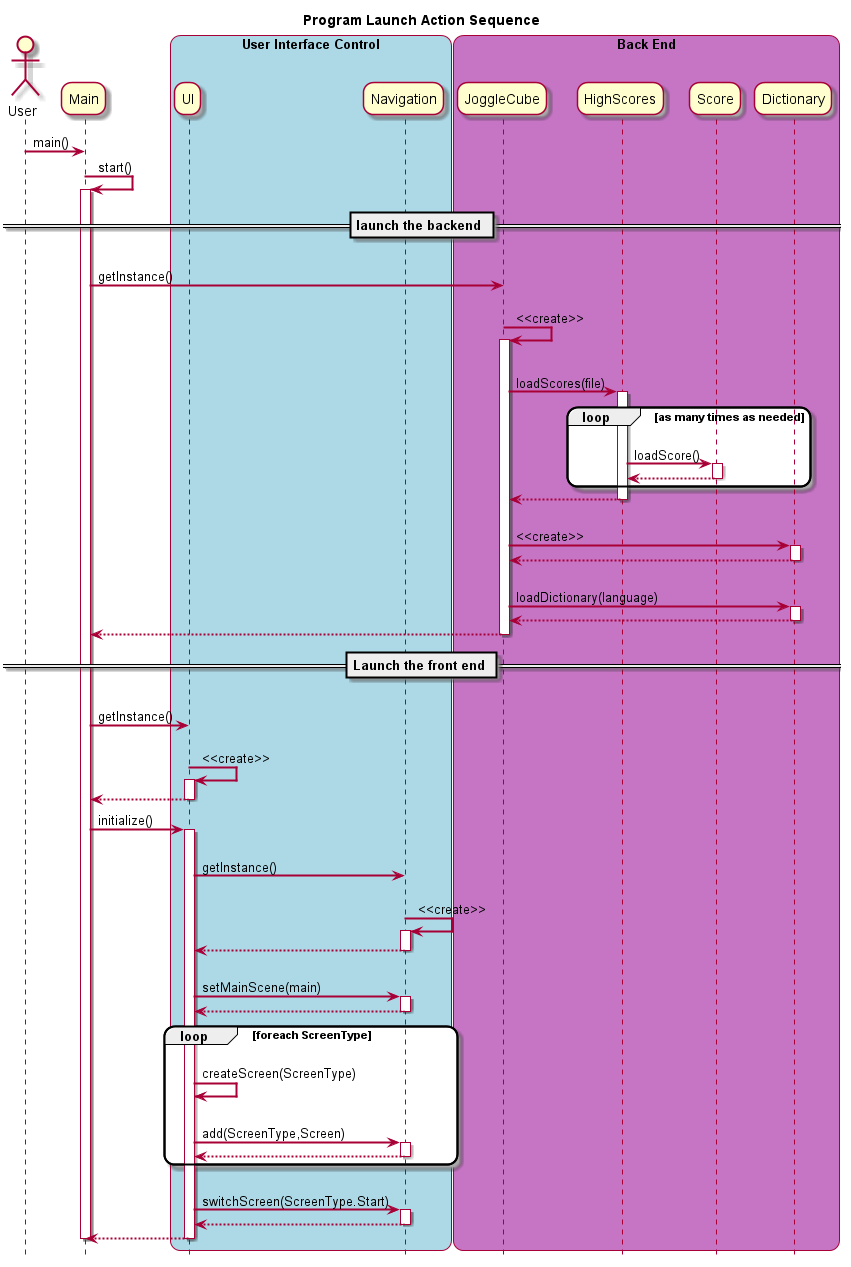
\includegraphics[width=15cm]{Main}
        \newpage
    	\subsubsection{UI}
            \paragraph{Start}
        		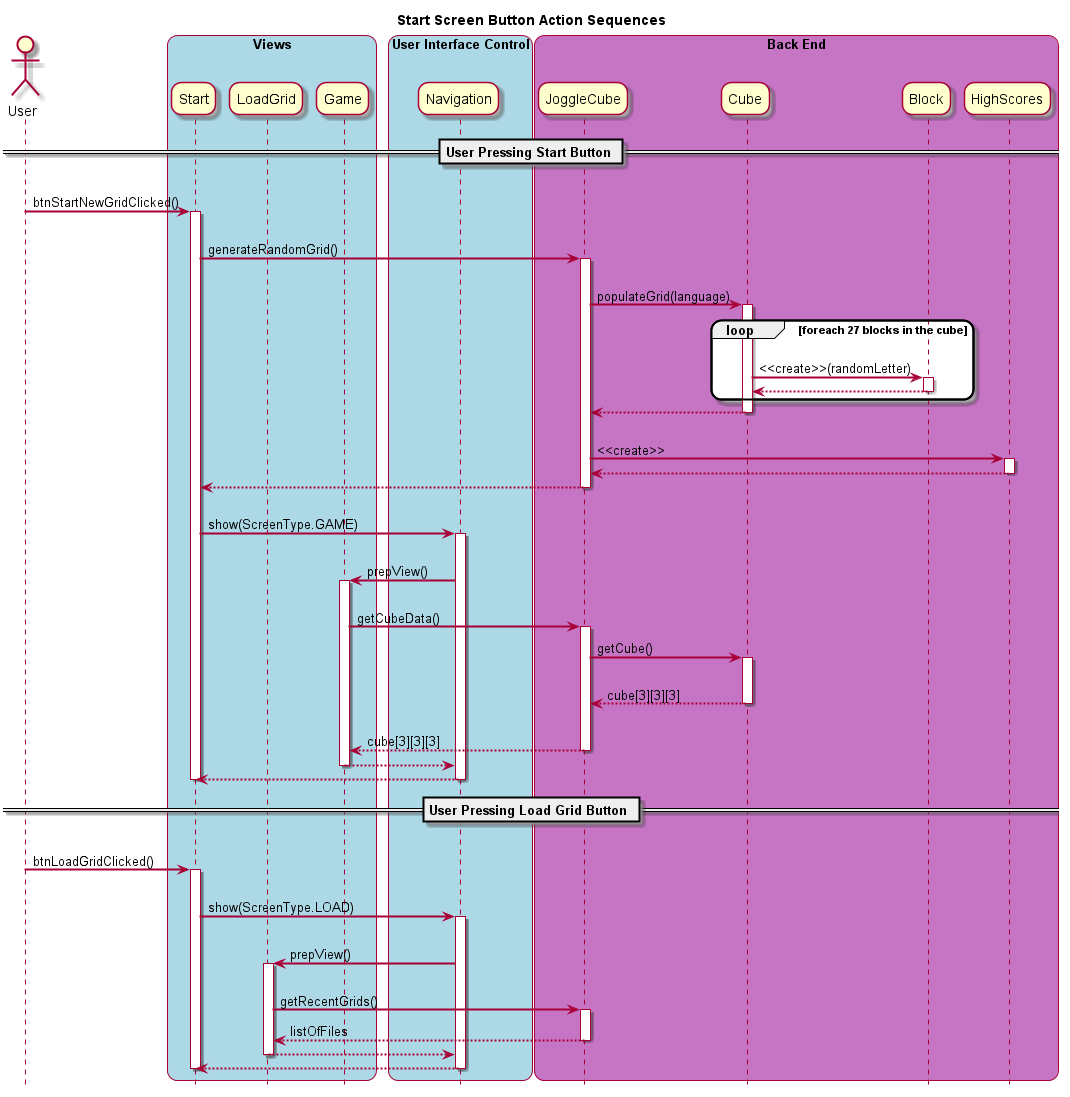
\includegraphics[width=17.5cm]{Start}
                \newpage
            \paragraph{LoadGrid}
            	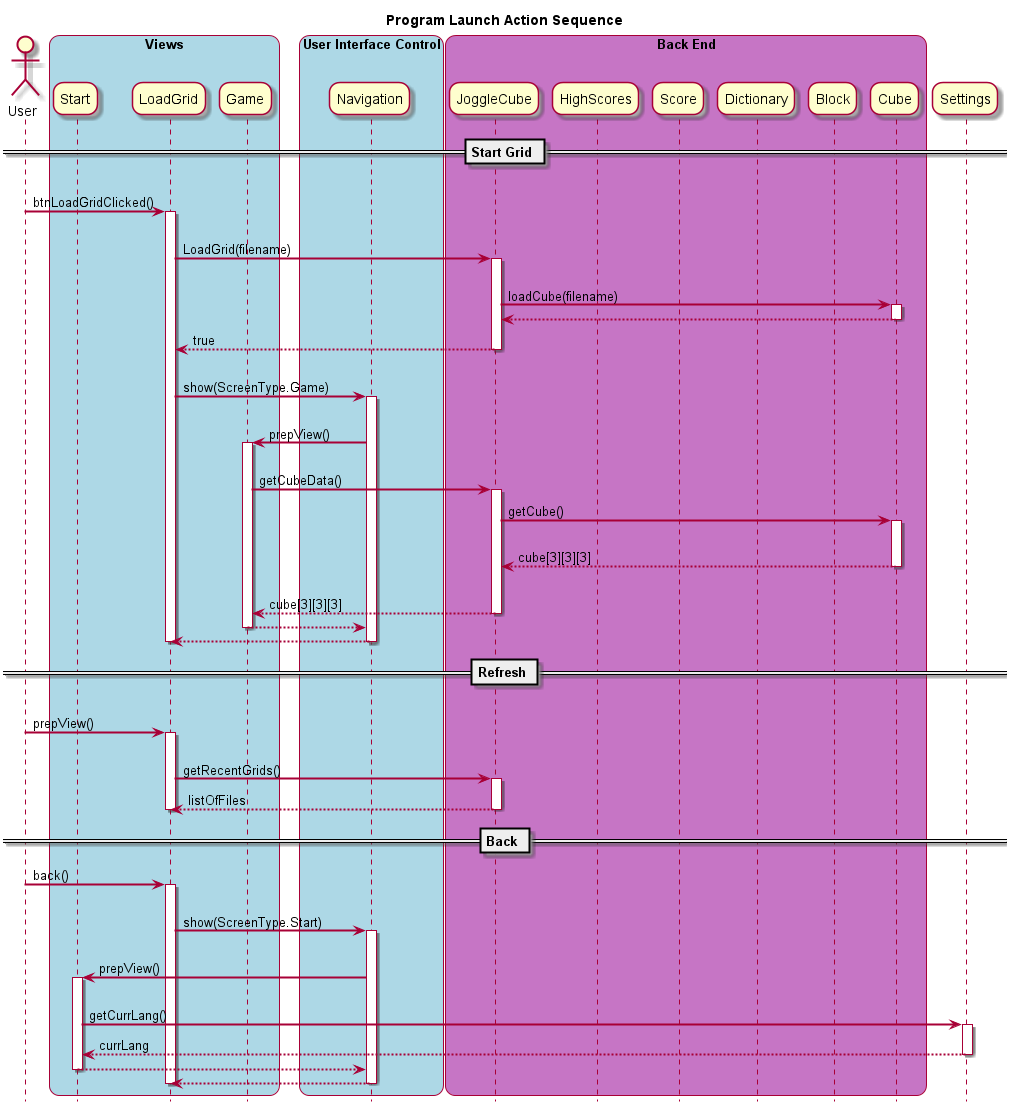
\includegraphics[width=17.5cm]{Load}
                \newpage
            \paragraph{Game}
            	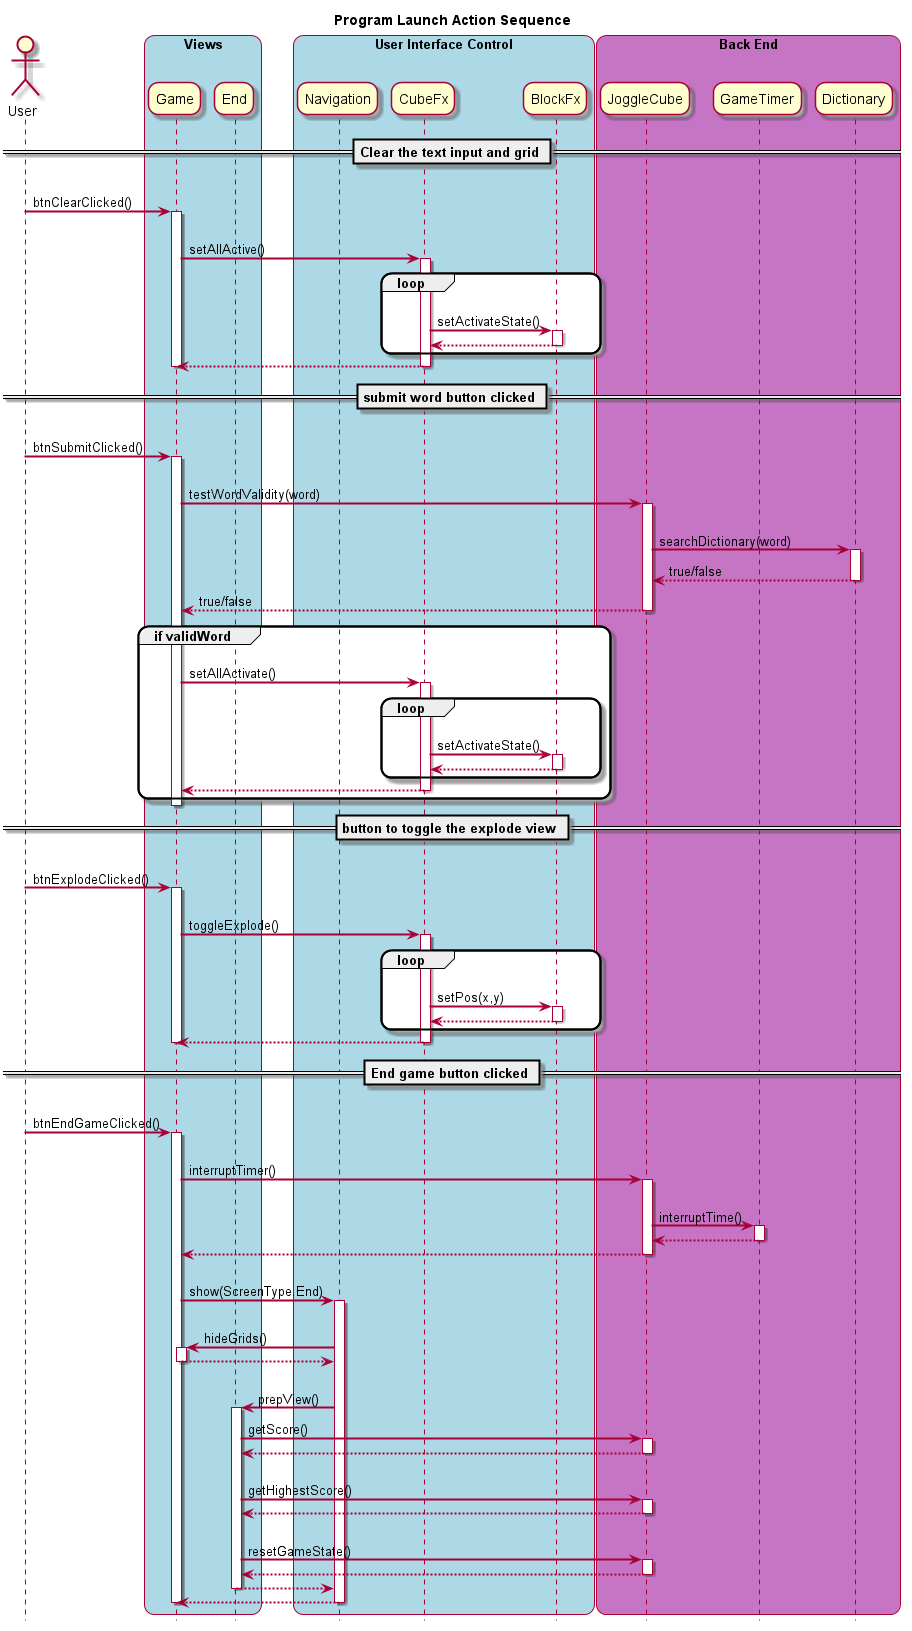
\includegraphics[width=13.5cm]{Game}
                \newpage
            \paragraph{End}
            	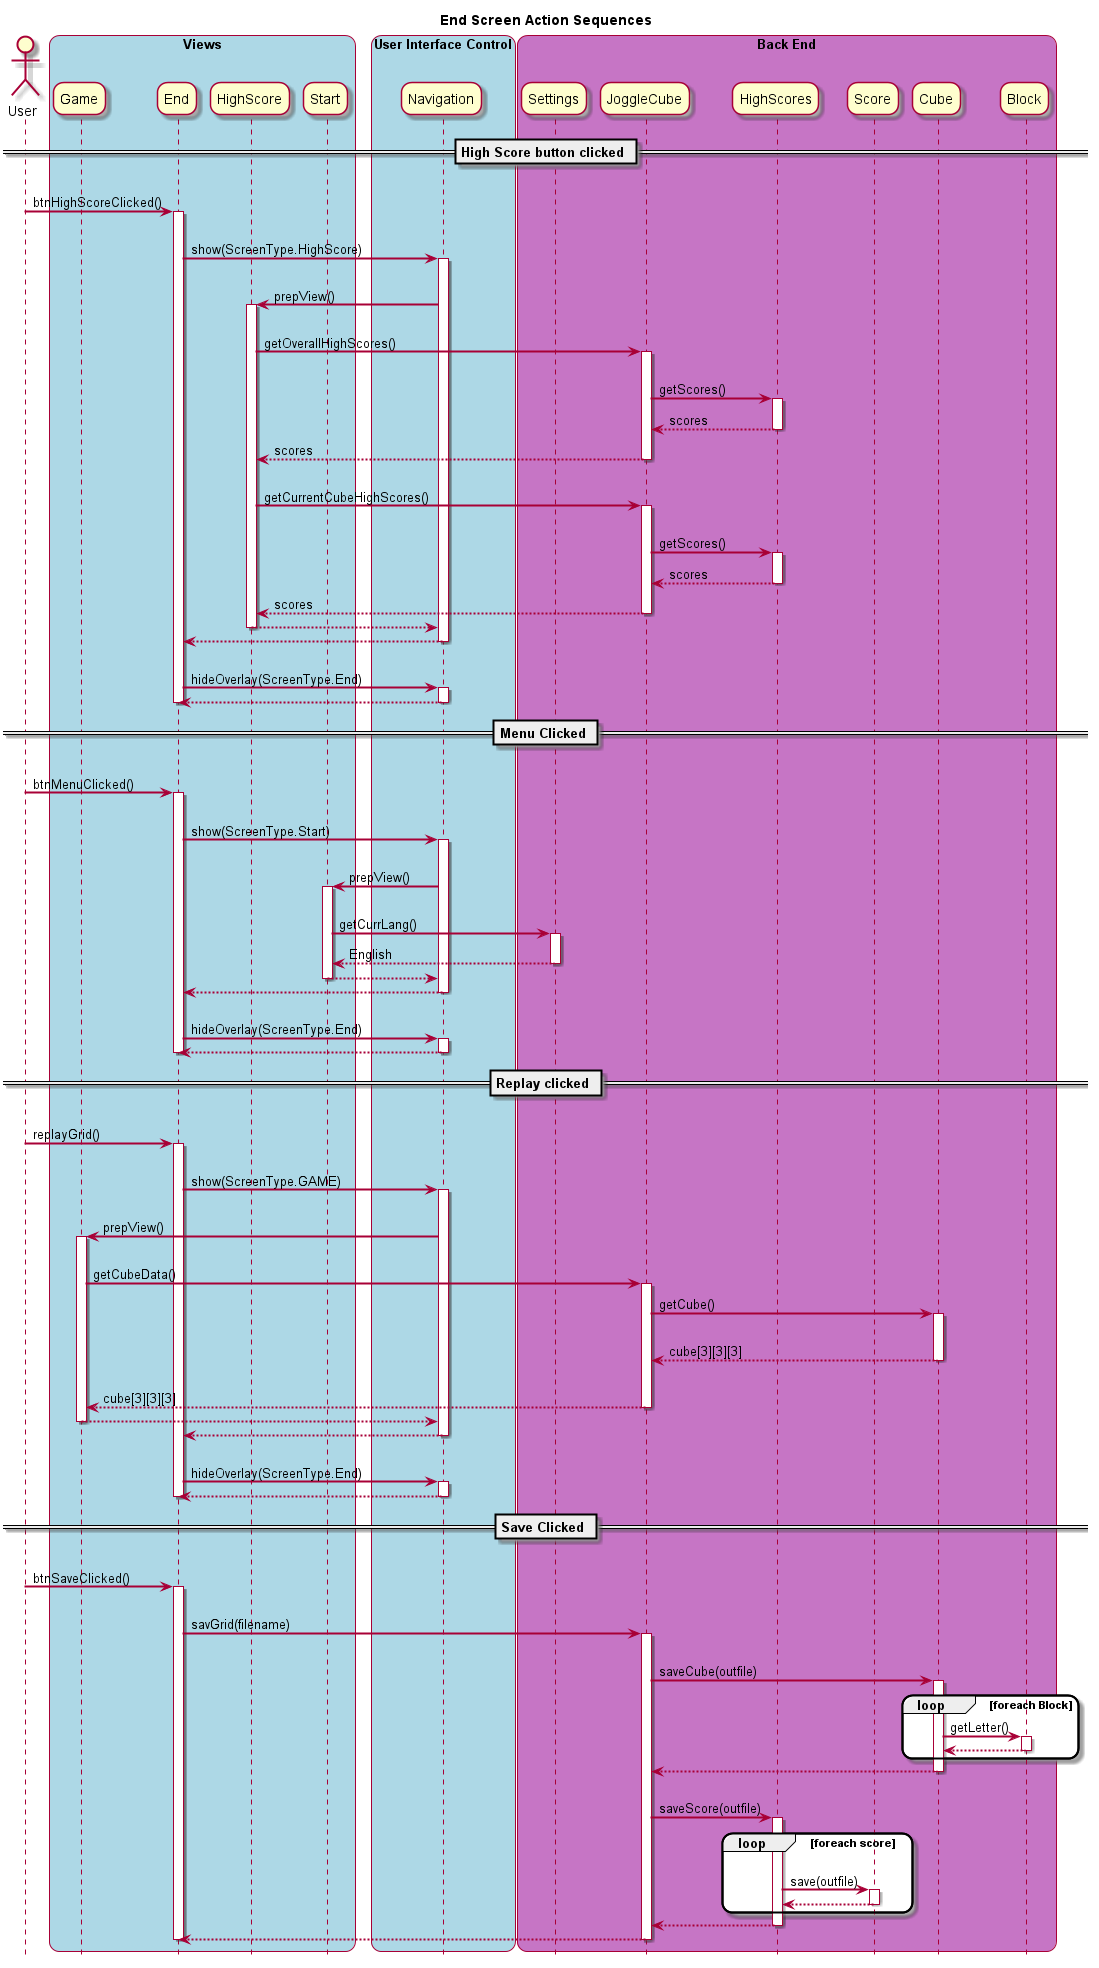
\includegraphics[width=13.5cm]{End}
                \newpage
            \paragraph{BaseScreen}
            	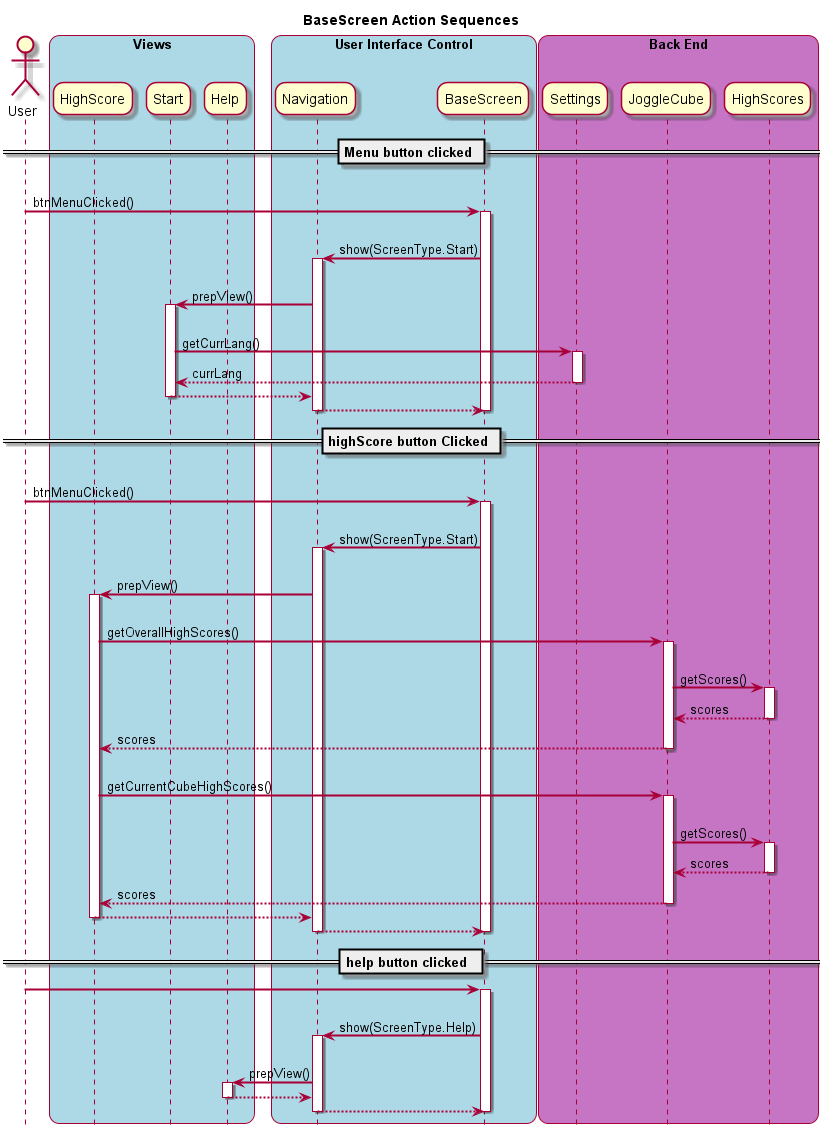
\includegraphics[width=\textwidth]{BaseScreen} % Nathan - DONE
    \newpage
    \subsection{Significant algorithms} %Leave this Sam and Nathan
    \subsubsection{Dictionary Load}
    Dictionary loading is an algorithm that is actually fairly short in nature but requires very specific elements to be efficient, to allow for the Dictionary to be built quick enough. This is achieved by utilizing the HashMap data structure in the Java standard library. This is achieved by feeding the given file name into the function and then the algorithm will find the file name given in the resources folders of the project. At this point it will read the entire contents of the file into the HashMap<String, String> data structure, the HashMap uses the key and value as the same String input, the string input is the word that is being added to the dictionary.
    
    This function took some testing to get the design right, it was tested by having the load time being calculated and displayed in the console. The load times on machines that I had tested it on never gets over 600ms to any significant degree (170,000+ words present), so the dictionary loading did not require a load screen before the main menu, so to stop the functional requirement of things happening within 1 second of an action happening being broken.
    
    This particular algorithm should be called in the overall back-end JoggleCube class whilst the algorithm is written in the Dictionary class.
    \subsubsection{Dictionary Search}
    Dictionary search was the part of the program that had to most crucially be performed quickly. If the search was slow it would be noticeable in the game and that leads to the main design decision of loading the dictionary into a HashMap of String key-value pairs where the key and the value are both strings. This algorithm is to be called every time the player submits a word so it was critical that it was fast.
    
    The search should be achieved by entering a word into the method and returning true if the word is in the dictionary HashMap structure, or false if it is not. It requires no further data and the actual search of the HashMap is handled by the Java Standard Library implementation of HashMap.
    
    This algorithm is called in the JoggleCube class when testing the validity of an entered word against known statistics. The actual algorithm is present in the Dictionary Class.
    \subsubsection{Finding neighbouring blocks/Is a neighbour}
    Finding which blocks are neighbouring other blocks was surprisingly hard to calculate at least initially. The original design was meant to take each block and decide whether or not it is a neighbour iterating through all other potential blocks. The runtime for this was much higher than the design we finally settled on after giving it more thought. The algorithm we settled on would calculate the potential neighbours of a block by generating each of the potential 27, neighbours I check to see if they are valid block numbers and if they are then they are returned as a neighbour of that block.
    
    The function was originally designed to be a backend feature feeding an ArrayList of coordinates, however, it is adapted into a front-end version to help with the grid displayer.
    
    The algorithm was originally meant to work in the Cube class and the adapted version was written in the front-end version. The actual algorithm was implemented in the Grid Displaying class.
    \subsubsection{Saving Grids} \label{SaveGrid}
    The act of saving the grid requires a filename to be given as a string into the algorithm which will take the current cube, current language and current cube high scores and save it in the appropriate grid format, this is discussed in Section: \ref{CubePersistance}. Then after creating the file, it prints out the language of the current state of the cube/game. Then it feeds the file into the saveCube method which handles it saving in the right order and format previously discussed, then it feeds the same file pointer into the saveScores method of HighScores which is discussed also in Section: \ref{Scores}. After that, it closes the file and thus the file is saved.
    
    The function handles the saving of a grid in it's current state to the saves folder made at program startup if not already present in the documents folder of the current machine user.
    
    This algorithm is called whenever the user asks to save the grid, on the front-end, however, the algorithm itself is present in JoggleCube the main backend class.
    \subsubsection{Loading Grids} \label{LoadGrid}
    To load a grid much like saving a grid it requires a filename to be given as a string into the algorithm. Then the file is opened by the program and the data is read in respectively in a way similar to how it was saved. It reads in the language of the file and then sets the current language to that in the settings. Then the file is feed into loadCube in the cube class which causes the cube data to be loaded in, then that same file is given to the loadScores in Scores class. The way the cube and high scores for that cube are loaded is relevant to the way they should be saved and thus can be found in Sections: \ref{CubePersistance} and \ref{Scores}. At this point, the saved state of the game has replaced all relevant parts of the program so that the new Cube has been fully loaded.
    
    The function handles loading of a new cube/grid, the high scores and the language of the saved data.
    
    This algorithm is called on the front-end, but the actual algorithm is only present in the JoggleCube main back-end class.
    \subsubsection{Random Letter Generation}\label{RandomLetter}
    Random Letter Generation is accomplished by utilising a 'Bag of Letters'. The Letters are stored in an ArrayList<String>. So the algorithm loads in the 'Bag of letters' from a file containing the number of letters correlating to the abundance of the letters given in the functional requirements or if it's not English we will base it from the basic scrabble rules of that language. Then it generates a random number using this random number it takes the letter from the array list and removes it from the list, at that point it is put into the cube at the first position [0][0][0] and then it iterates by one on the first to put another random letter in to [0][0][1] and so on until it iterates up to two on each part of the modelled cube, until 27 unique positions in the array have been used and pseudo-randomly generates the cube.
    
    The function in question will populate the entire cube with random letters in Block objects utilising the random function built into Java the cube should be entirely random, using the weightings given in the functional requirements. This is a backend function which is used to create the cube.
    
    The algorithm should be called in the JoggleCube class where the cube is present to regenerate the cube into a new random cube as well as once at startup. However, the actual algorithm is present in the Cube class.
    \subsubsection{Creation of JoggleCube in documents folder}
    The JoggleCube program requires a place to saved files locally that isn't in the game files itself, it needs this as we want to package the program into a .jar Java file so we can give it out to be people to test the game for us and so we can easily test it on different machines. Therefore the design decision was taken to store saves and the overall scores for high scores locally on the machine in the documents folder, regardless of the operating system used. This can be achieved by finding the local system home and navigating to the documents folder. If in the documents folder the JoggleCube folder has already been created then do nothing. If it hasn't we want it to create the JoggleCube folder, the saves folder inside of that folder and a high score folder for housing the saves and overall high scores for this user account respectively. Then we want to create the overAll.highscores file and copy three example grid saves into the saves folder.
    
    The function in question will make sure that the files are present for the program when it needs them as well as making sure that the saves can be saved locally, also saving the high scores locally. This stops potential errors when looking for these files, later in the program.
    
    The algorithm should be called in JoggleCube when the JoggleCube object is created and this is a private method to stop it being called outside of this class.
    \subsubsection{Recent Grids}
    The recent grids algorithm should check the documents on the computer for the saves that were saved locally, and return an ObservableList<String> of the names of these files without the .grid extension. It should accomplish this by getting a list of all files in the saves folder in an array of File[]. Then we add the names of the files to an ArrayList<String> to store the full name of the file including the file extension, .grid. Then using this ArrayList we will process each part of the list individually using a StringBuilder to remove the .grid file extension and add it to a new ObservableList<String> so we can return it. We didn't originally put things in the ObservableList as it is harder to process data in this list than an ArrayList. Then return this new ObservableList so it can be displayed on the front-end class that called it.
    
    This function will make it easy for people to load any grid they have saved, as all saved grids will be displayed in this list.
    
    The algorithm should be called on the front-end, and the actual algorithm should be present in the JoggleCube class on the back-end of the program.
    
    \subsubsection{Displaying the Grids} %Nathan
    The grid displaying is going to be done using two classes: CubeFx and BlockFx. Where BlockFX will store a label, two blocks and 4 materials for each possible state of the Block, the block will then have 4 possible states in which it can be. CubeFx will take a 3-dimensional cube of letters and generate its own internal 3-dimensional cube of BlockFX's for display. The CubeFx class will also handle exploding the 3d cube using java's timeline library to animate it.
    
    \subsubsection{Loading overall High Scores}
    The way we load overall highscores is very similar in some aspects to how we load a grid just there isn't a grid to be loading. The overall highscores loads in the data by calling loadScores in the Scores class by finding the overall highscores in the previously made folder in the documents folder, the file itself should be called overAll.highscores. The returned ArrayList from the loadScores method should then be set as the overHighscores instance variable in JoggleCube so it can be used in other methods down the line.
    
    This function should be called on program startup. The algorithm should be present in the JoggleCube class and should be called at either the constructor of JoggleCube or during Main.
    
    \subsubsection{Word Score Generation}\label{WordScore}
    Word Score Generation is accomplished by feeding in a word as a String, into the method. then we will analyse the word letter by letter utilising the scores HashMap that was created when the grid was loaded with the "Bag of Letters" was loaded. The scores HashMap is a key-value pair data structure that utilizes the letter as the Key and the score associated with that letter as the value. Using this previously constructed data structure, we can search for the value of the letter at each point of the word, by searching the HashMap. At first, we check whether the letter and the letter following it make up a double letter in the HashMap, if they do we increment the search loop by 1 to emulate that extra letter and then we add the score of that pair to the int variable that is used to handle the total score. If the letter is not part of a pair, it then checks if that letter is a valid letter by itself and if it is, it then will add the score of that letter to the overall sum. If neither of these checks works then there is an error in the scores loaded from the file and an error should be handled. At this point, we then return the value squared, as the scores that are saved/loaded are the given values for the letters of scrabble.
    
    The function in question will return the score as an int to the place that called it. This is another backend function which is used to update the backend values of the score and display the new score on the front-end GUI display.
    
    The algorithm should be called in the JoggleCube class the main backend class that handles most of the algorithm decisions. The actual algorithm is also present in JoggleCube and thus it can be handled as a private method as it isn't needed to be called in other classes. However, if we decided to add in extra features such as word score display for the word during the game the function could be made public and called.
    \subsubsection{Test Word Validity}
    Test Word Validity is accomplished by first of all checking whether the word has already been checked and successfully added to the list of previously used words, this list of previously used words is added to when this function is about to return true, so if the word has already been checked and it returned true then the function would return false, as this word is not valid. The next check that occurs is actually checking whether it is a valid word in the dictionary of the language that is currently being used (Default is American English (There was no easy to access a large dictionary of British English Scrabble legal words that we could find)). If it is a word that has appeared in the dictionary then the current score of the game is updated using word score generation, the game score label is updated on the front end and the word that is checked against is added to the aforementioned stored words list. Then the function should return true, else if it is not in the loaded dictionary it returns false.
    
    The function in question will take in the String word and return true if the word is valid and update the relevant data sets or it will return false if it is not valid and update nothing.
    
    The algorithm should be called from the front-end class that is handling the processing of words entered when the submit button is pressed. However, the actual algorithm is present in the main JoggleCube back-end class. % Sam and Nathan- DONE - NEEDS REVIEW FOR GRAMMAR AND PUNCTUATION
    \newpage
    \subsection{Significant data structures}
\subsubsection{The UML Class Diagram}
\begin{sideways}
        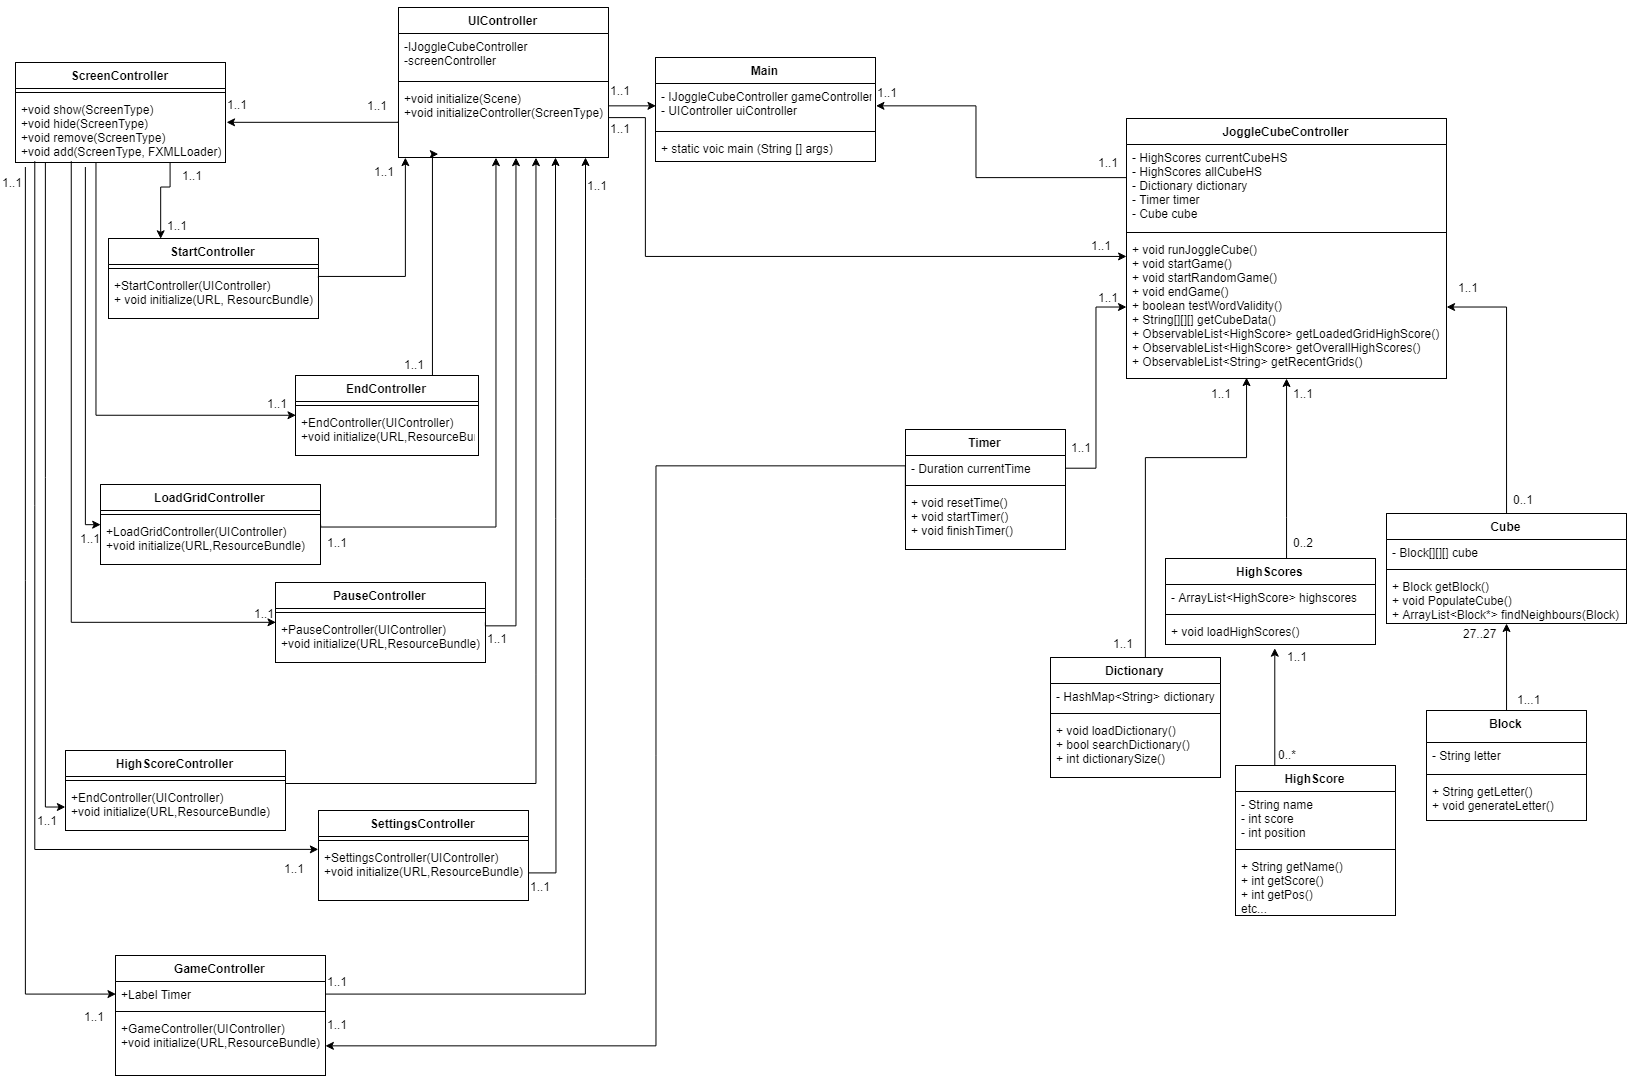
\includegraphics[width=22cm]{Layout_-_drawio_save_ver5_2}
\end{sideways}
        \newpage
    \subsubsection{Object Diagram}
        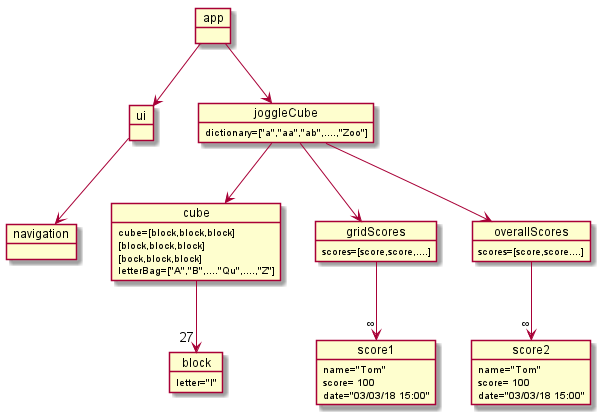
\includegraphics[width=\textwidth]{Cube}
    \subsubsection{Data Persistance}
        \paragraph{Dictionary}
        The way in which Dictionary is kept persistent between program uses is by utilising a text file with no extension. Each dictionary of the program has a very specific layout that must be followed. The document needs to have a word in it for every line, but only one word on each line, if you have 70 words total then you have 70 lines containing one word each. The case of the word doesn't matter as it is handled to take both. The way different dictionaries are loaded is by having the first two characters of the filename be two characters that represent the language e.g. English = en\_dictionary and Welsh = cy\_dictionary.
        
        An example of this can be found in Appendix \ref{DictionaryExample}
        \paragraph{LetterBag}
        The LetterBag needs to be loaded from a specific file with a specific name, the name is parsed similarly to the dictionary in the sense that the naming scheme for English is en\_letters. The letter bag then has one line per letter, the letter is followed by a space then how many times that letter can be "pulled out of the bag" or used in the cube, then it is followed by another space and the score in scrabble not the JoggleCube game (this is applied later). Then the line ends and the next letter happens with the same things after it. e.g. "A 9 1" - is the first line in en\_letters, this also handles Double letters as one so you have Qu represented as "QU 1 8" as a line in the English letter bag. This allows for different languages to be loaded in using the current framework so it's relatively simple to expand the game's language base. The way the LetterBag file is processed by the program has already been discussed earlier in Sections \ref{RandomLetter} and \ref{WordScore}
        
        An example of this can be found in Appendix \ref{LetterBagExample}
        \paragraph{Cube}\label{CubePersistance}
        The Cube is interesting as you need to save the language of that cube to make sure that the correct dictionary and score lists are loaded. The first line of the Cube save files is the language representing by a 2 character string e.g. "en" for English. The next part of the file is the Cube itself, which is 9 lines of 3 characters with spaces between them to represent the grid. This is for visualisation of the cube in the files, with the first character being [0][0][0] and the last being [2][2][2] etc. The Cube then still has its specific high scores to be loaded in which are saved in the Format "Date Time Score Name" with spaces as a delimiter between each value. Further examples of the score can be found in Appendix \ref{HighScoresExample}. The way this file is actually parsed and brought into the program is discussed in Sections: \ref{LoadGrid} and \ref{SaveGrid}
        
        An example of the Cube can be found in Appendix \ref{CubeExample}
        \paragraph{(High) Scores}\label{Scores}
        The (High) Scores part is interesting because it needs to be saved in both Cubes and overAll.highscores and the way this was achieved is with a framework for saving it. The way this is handled for Cubes is described in section \ref{CubePersistance}. The way overAll.highscores is kept persistent is similar to grids but it saves when the program exits or when a grid is finished, and without the grid and language definitions. So it's a long file with one set of HighScores per line with the format "Date time Score Name" e.g. "2018/03/14 15:40 87 player87".
        
        An example of the High Scores can be found in Appendix \ref{HighScoresExample} whilst the way in which individual cubes handle their high scores are discovered in Appendix \ref{CubeExample} % Sam and Nathan - DOING - NEEDS REVIEW FOR GRAMMAR AND PUNCTUATION % Nathan - UML Sequence and Object + Sam - UML Class diagram, Algorithms and Data Persistence.
    \begin{appendices}
\section{Dictionary Example} \label{DictionaryExample}
    A dictionary file might look something like this:\newline
    APRON\newline
    BARBECUE\newline
    CHILLI\newline
    DANDELION\newline
    EGG\newline
    FRY\newline
    GRASS
    
    All of these words would be loaded in and handled as a dictionary in a HashMap.
\section{LetterBag Example} \label{LetterBagExample}
    A LetterBag file might look something like this:\newline
    A 9 1\newline
    B 2 3\newline
    C 2 3\newline
    D 4 2\newline
    E 12 1\newline
    F 2 4\newline
    G 3 2\newline
    H 2 4\newline
    I 9 1
    
    So, for example, A would be loaded into the bag 9 times and the score associated on the backend would be 1, as that is the scrabble score, and so on for the rest of the file.
\section{Cube Example} \label{CubeExample}
    A saved Cube/Grid might look something like this:\newline
    en\newline
    E R T\newline
    L A P\newline
    O Qu T\newline
    M N B\newline
    L A P\newline
    A U I\newline
    Z M A\newline
    Y T R\newline
    D F G
    
    This is a Cube without any current high scores, but the cube is in English and the position [0][0][0] is E whilst [2][2][2] is G, it is set up to be easy to interpret from the file.
    \newline% The Appendix needed to go to the next page and I forgot the thing to automatically do it so I did this janky method - Sam
    \newline
    \newline
    \newline
    \newline
    
      However, the Cube/Grid file with scores might look something like this:\newline
    en\newline
    D O A\newline
    X R C\newline
    F E Z\newline
    W P A\newline
    E U I\newline
    S I V\newline
    E Y G\newline
    N L G\newline
    D J O\newline
    2018/03/14 22:42 591 James\newline
    2018/03/14 22:50 1744 Moses

    This shows that Moses got a score of 1744 on this grid at 22:50 on 14/03/2018. These scores are then loaded and visible but the way they are parsed is discussed in Section \ref{LoadGrid}
\section{(High) Scores Example} \label{HighScoresExample}
    The overAll.highscores file might look something like this:
    
    2018/03/19 15:59 1825 Walter\newline
    2018/03/14 22:50 1744 Moses\newline
    2018/03/14 22:42 591 James\newline
    2018/03/14 22:46 367 Jamie\newline
    2018/03/18 11:54 85 Walter

    You can see how there have been 5 games with a score greater than 0 that have been played on this user account of this machine at least since the last time overall scores were cleared.
    
    The other scores are handled exactly the same at the end of a Cube(Shown in Appendix \ref{CubeExample}) but you might see them in the file like this:
    
    2018/03/14 22:46 367 Jamie\newline
    2018/03/18 11:54 85 Walter
    
    This is obviously after the gid information and the format of saving the high score data is the same between overAll and all the grid's individual scores. This Cube has 2 scores where Jamie got a score of 367 at 22:46 on 14/03/2018 and Walter got a score of 85 at 11:54 on 18/03/2018.
\end{appendices} %Sam
	\addcontentsline{toc}{section}{REFERENCES}
	\begin{thebibliography}{5}
		\bibitem{SE.QA.CSRS} \emph{Software Engineering Group Projects}
JoggleCube Game Requirements Specification.
C. J. Price SE.QA.CSRS. 1.0 Release.
	\end{thebibliography}
	\clearpage
	\addcontentsline{toc}{section}{DOCUMENT HISTORY}
	\section*{DOCUMENT HISTORY}
	\begin{tabular}{| l | l | l | l | l |}
		\hline
		Version & CCF No. & Date & Changes made to Document & Changed by \\
		\hline
		0.1 & N/A & 2018-03-08 & Initial creation & NAW21 \\ \hline
        0.2 & N/A & 2018-03-19 & Filled with content & All \\
		\hline
	\end{tabular}
	\label{thelastpage}
\end{document}